\documentclass[11 pt,letterpaper]{article}
\usepackage{graphicx,float}
\usepackage[section]{placeins}
\usepackage[margin=1.5in]{geometry}
\usepackage[colorlinks=true,urlcolor=black]{hyperref}

\title{\LARGE \bf
    BIF705 Lab 2:\\
    Microarray Pre-Processing in R
    }
\author{Christopher Eeles}
\date{\small \today}

\begin{document}

\maketitle

\section{Introduction}
    In this report we will be analyzing a human gene expression profile of the ETS2 gene in lung cancer cells transfected with either scrambled siRNA or siRNA specific to ETS2.$^5$
    The original experiment was conducted using the Affymetrix GeneChip system, an industry standard technology for analyzing one-colour oligonucleotide microarrays which enables direct comparisons of expression levels across treatment conditions.$^1$$^,$$^4$
    In order to ensure accurate comparisons, probe intensity data from the GeneChips must be pre-processed to standardize across different arrays and probe sets.$^1$
    To facilitate such processing, as well as downstream analysis, the \textit{affy} package for the R programming language was developed as part of the larger Bioconductor suite of R bioinformatics software.$^3$
    
    Various statistical methods are available for data pre-processing, however, this analysis will utilize robust microarray analysis (RMA).$^1$
    This technique passes raw data through four major steps: background correction, quantile normalization, log2 data transformation and median polish error estimation.$1$
    Our current analysis will examine graphical differences between the raw and pre-processed ETS2 expression profile data using functions and methods from \textit{affy} and related R packages.$^2$
    In doing so we hope to visually demonstrate the importance of data pre-processing for valid downstream analyses, as well as explore some basic applications of the \textit{affy} package for cleaning, processing and visualization of gene expression data.

\section{Results}
    \subsection{Unprocessed}

    \begin{figure}[H]
        \centering
        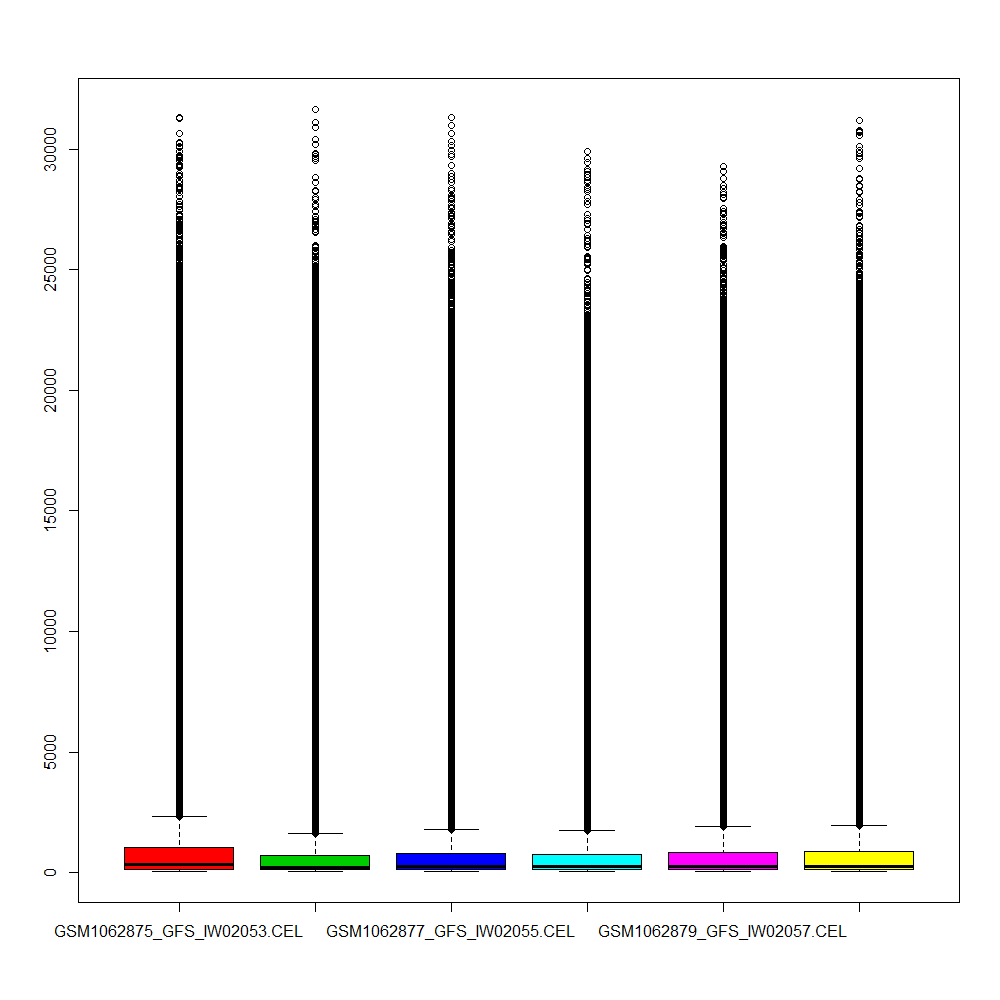
\includegraphics[width=\linewidth]{Figures/Rplot03.png}
        \caption{Box Plot of Raw Affymetrix Data}
        \label{fig:plot1}
    \end{figure}
    \FloatBarrier

    \subsection{Pre-processed}
    \begin{figure}[H]
        \centering
        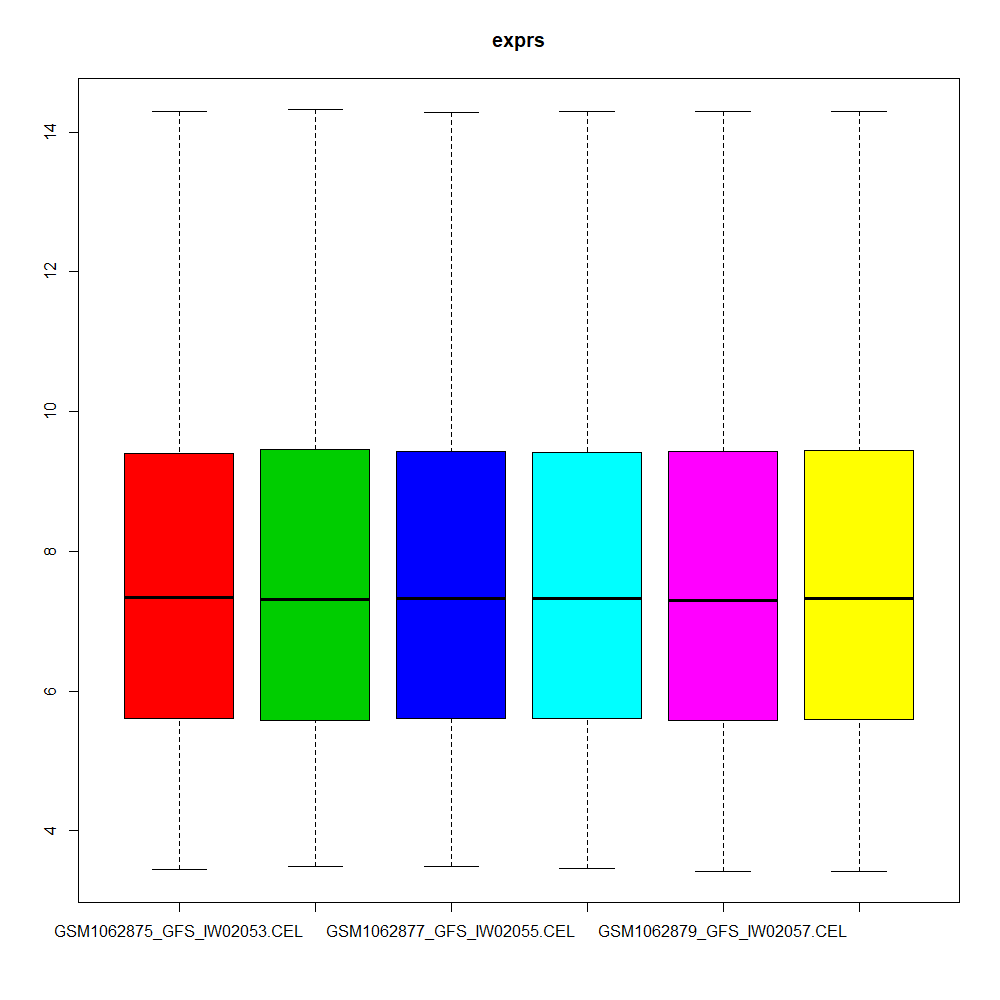
\includegraphics[width=\linewidth]{Figures/Rplot01.png}
        \caption{Box Plot of Pre-processed Affymetrix Data}
        \label{fig:plot2}
    \end{figure}
    \FloatBarrier

\section{Conclusion}

    Figure 1 and Figure 2 from the results section displays the box plots generating using \textit{affy} and other R packages available from the Bioconductor suite of software.
    The figures show intensity and log2(intensity), respectively, on the y-axes with both sets of x-axes representing GeneChips for different treatment conditions (\textit{i.e.}, scrambled vs targeted siRNA).
    From left to right, the first three plots are treatments with scrambled siRNA, while the remainder are treatments are with ETS2 targeted siRNA.
    The raw data in Figure 1 one is highly skewed and rich with outliers.
    Though it is difficult to see, the plot means and standard deviations are also unequal between GeneChips.
    Since the box plots represent the distribution of intensities for each GeneChip, the differences in distribution preclude comparison between GeneChips.
    
    Application of the \textit{affy} RMA function has resulted in significantly cleaner data, firstly by shrinking the y-axes via log2 transformation and secondly by normalizing across GeneChips.
    While the distributions still display a slight skew towards higher intensities, the mean and standard deviations between box plots are now approximately equal. 
    As such, downstream analyses are now able to make valid statistical comparisons between the GeneChips and therefore be confident in the resulting biological interpretations of the data.
    For future analyses it would be useful gain a better understanding of the objects, classes and methods available within the \textit{affy} package to allow inclusion of additional information about each GeneChip in the plots.
    For example, addition of axis labels, modification of plot titles, and implementation of more descriptive x-axis values could maximize the information communicated in generated visualizations.
    This will be a focus for further analysis using the \textit{package} as well as R packages more generally.

\begin{thebibliography}{1}

    \bibitem{1} School of Biological Sciences and Applied Chemistry. (2019). Pre-Processing of Gene Expression Data. Seneca College: Toronto, ON.

    \bibitem{2} School of Biological Sciences and Applied Chemistry. (2019). Microarray Pre-Processing in R. Seneca College: Toronto, ON.

    \bibitem{3} Gautier, L., Irizarry, R., Cope, L., and Blostad, B. (2018). Description of affy. Bioconductor [website]. Retrieved from \url{https://bioconductor.org/packages/release/bioc/vignettes/affy/inst/doc/affy.pdf}
    
    \bibitem{4} Gautier, L., Irizarry, R., Cope, L., and Blostad, B. (2003). affy-analysis of Affymetric GeneChip data at the probe level. Bioinformatics 20(3). Retrieved from \url{https://academic.oup.com/bioinformatics/article/20/3/307/185980}

    \bibitem{5} NCBI. (2013). GSE43459. Gene Expression Omnibus [website]. Retrieved from \url{https://www.ncbi.nlm.nih.gov/geo/query/acc.cgi}

\end{thebibliography}

\end{document}